\section{Architecture}

\begin{frame}{Summarizer Architecture}
  \begin{center}
    \begin{tikzpicture}
      \node at (0.4,-.75) {Sentence 1};
      \node at (4.9,-.75) {Sentence 2};
      \node at (8.9,-.75) {Sentence 3};
      \node (w1) at (0,0) 
      {\large $\uncover<2->{\textsc{Enc}\left(}w^{(1)}_1,
         w^{(1)}_2, w^{(1)}_3\uncover<2->{\right)}$};

      \node (w2) at (4.5,0) 
      {\large $\uncover<2->{\textsc{Enc}\left(}w^{(2)}_1, 
         w^{(2)}_2, w^{(2)}_3\uncover<2->{ \right)}$};
      \node (w3) at (8.6,0) 
      {\large $\uncover<2->{\textsc{Enc}\left(}w^{(3)}_1, 
         w^{(3)}_2\uncover<2->{\right)}$};

      \node (s1) at (3,2) {\large $\uncover<3->{s_1}$};
      \node (s2) at (4,2) {\large $\uncover<3->{s_2}$};
      \node (s3) at (5,2) {\large $\uncover<3->{s_3}$};
      \uncover<3->{  
        \draw[->,thick] (w1.north) -- (s1.south); 
        \draw[->,thick] (w2.north) -- (s2.south);
        \draw[->,thick] (w3.north) -- (s3.south);
      }

      \uncover<4->{
        \node (ext) at (3.6,2) {\large $\textsc{Ext}\Big( 
        \quad\quad\quad\;\;\;\;\;\;\;\;\;\;\; \Big)$};
      }
      \uncover<5->{
        \node (y1) at (3,3.5) {\large $y_1$};
        \node (y2) at (4,3.5) {\large $y_2$};
        \node (y3) at (5,3.5) {\large $y_3$};
        \draw[->,thick] (s1.north) -- (y1.south);
        \draw[->,thick] (s2.north) -- (y2.south);
        \draw[->,thick] (s3.north) -- (y3.south);
      }

    \end{tikzpicture}
  \end{center}
\end{frame}


\begin{frame}{Sentence Encoders}
 \begin{columns}[t]
  \column{.32\textwidth}
   \centering
   Averaging Encoder\\~\\
   \includegraphics[]{images/avg_encoder.pdf}\\
  \column{.32\textwidth}
   \centering
   RNN Encoder\\~\\
   \includegraphics[]{images/rnn_encoder.pdf}\\
  \column{.32\textwidth}
   \centering
   CNN Encoder\\~\\
   \includegraphics[]{images/cnn_encoder.pdf}\\
 \end{columns}

~\\
  Word embeddings are fixed Glove embeddings (trained on Wikipedia and 
    Gigaword). 

\end{frame}
%
%\begin{frame}{Sentence Extractor}
%  \textbf{Previous Work}\\~\\
%  ~~ -- \textbf{Cheng and Lapata Extractor} ~~ seq2seq inspired architecture 
%                                               (Cheng and Lapata, 2016)\\
%  ~~ -- \textbf{SummaRunner Extractor} ~~ RNN inspired architecture with 
%                                          document and summary representations 
%                                          (Nallapati et al., 2016)\\
%  ~\\~\\
%  \textbf{Our Extractors}\\~\\
%  ~~ -- \alert<2>{\textbf{RNN Extractor}} ~~ Simplified version of SummaRunner \\
%  ~~ -- \textbf{Seq2Seq Extractor} ~~ seq2seq (with attention) inspired 
%                                      architecture \\
%\end{frame}


\begin{frame}{Sentence Extractors}
 \begin{columns}[t]
  \column{.4\textwidth}
   \centering
   SummaRunner Extractor\\
   (Nallapati et al. 2016)\\
   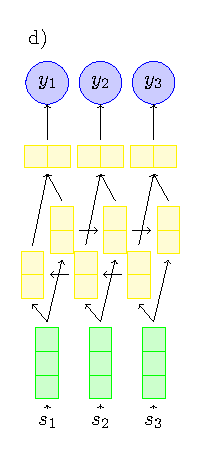
\includegraphics[scale=.65]{images/sr_extractor.pdf}\\
   RNN Extractor (ours)\\
   \includegraphics[scale=.65]{images/rnn_extractor.pdf}

  \column{.6\textwidth}
   \centering
   Cheng \& Lapata Extractor\\
   (Cheng and Lapata, 2016)\\
   \includegraphics[scale=.65]{images/cl_extractor.pdf}\\
   Seq2Seq Extractor (ours)\\
   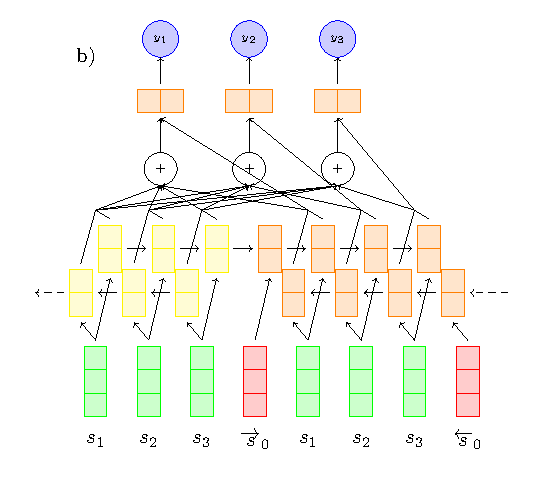
\includegraphics[scale=.65]{images/s2s_extractor.pdf}
 \end{columns}

\end{frame}


%\begin{frame}{Sentence Encoder}
%  \textbf{Averaging Encoder} ~~ $s = $ average of word embeddings \\
%  ~\\
%  \textbf{RNN Encoder} ~~ $s = $ final states of bi-directional GRU.\\
%  ~\\
%  \textbf{CNN Encoder} ~~ $s = $ 1-d convolutions over word embeddings.\\
%  ~\\~\\
%  * Word embeddings are fixed Glove embeddings (trained on Wikipedia and 
%    Gigaword). 
%\end{frame}
%

%
%\begin{frame}{RNN Extractor}
%  \begin{columns}
%    \begin{column}{0.5\textwidth}
%      \documentclass[crop,tikz]{standalone}
\usetikzlibrary{shapes}
\usetikzlibrary{arrows}
\usetikzlibrary{positioning}

\begin{document}
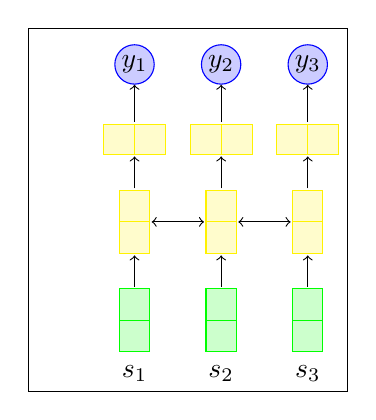
\begin{tikzpicture}[
  hid/.style 2 args={
    rectangle split,
    draw=#2,
    rectangle split parts=#1,
    fill=#2!20,
    outer sep=.25mm},
  mlp/.style 2 args={
    rectangle split,
    rectangle split horizontal,
    draw=#2,
    rectangle split parts=#1,
    fill=#2!20,
    outer sep=.25mm}
]

 % Comment out this line to remove border.
 \draw[draw=black] (-.25, 4.21) rectangle (3.8, -.4);

 \foreach \step in {1,...,3} {
   \node (i\step) at (1.1*\step, -.18) {$s_\step$};
   \node[hid={2}{green}] (e\step) at (1.1*\step, .5) {};    
 }
  
 \foreach \step in {1,...,3} {
   \node[hid={2}{yellow}] (h\step) at (1.1 *\step, 1.75) {};    
   \draw[->] (e\step.north) -> (h\step.south);
   
   \node[mlp={2}{yellow}] (g\step) at (1.1 *\step, 2.8) {};    
   \node[circle, draw=blue, fill=blue!20,minimum size=5mm] (y\step) 
       at (1.1 *\step, 3.75) {};
   \node at (1.1 *\step, 3.75) {$y_\step$};    
   \draw[->] (g\step.north) -> (y\step.south);
   \draw[->] (h\step.north) -> (g\step.south);
 }

 \foreach \last/\next in {1/2, 2/3} {
   \draw[<->] (h\last.east) -> (h\next.west);
 }


\end{tikzpicture}
\end{document}

%    \end{column}
%    \begin{column}{0.5\textwidth}
%      \uncover<2->{
%            $p(y|h) = \prod_{i=1}^n p(y_i|h)$ 
%      }
%    \end{column}
%  \end{columns}
%\end{frame}
%
%\begin{frame}{Sentence Extractor}
%  \textbf{Previous Work}\\~\\
%  ~~ -- \textbf{Cheng and Lapata Extractor} ~~ seq2seq inspired architecture 
%                                               (Cheng and Lapata, 2016)\\
%  ~~ -- \textbf{SummaRunner Extractor} ~~ RNN inspired architecture with 
%                                          document and summary representations 
%                                          (Nallapati et al., 2016)\\
%  ~\\~\\
%  \textbf{Our Extractors}\\~\\
%  ~~ -- \textbf{RNN Extractor} ~~ Simplified version of SummaRunner \\
%  ~~ -- \alert{\textbf{Seq2Seq Extractor}} ~~ seq2seq (with attention) inspired
%                                              architecture \\
%\end{frame}
%
%
%
%\begin{frame}{Seq2Seq Extractor}
%    \begin{columns}
%        \begin{column}{0.5\textwidth}
%            \documentclass[tikz,border=10pt]{standalone}
\usetikzlibrary{shapes}
\usetikzlibrary{arrows}
\usetikzlibrary{positioning}
\begin{document} 

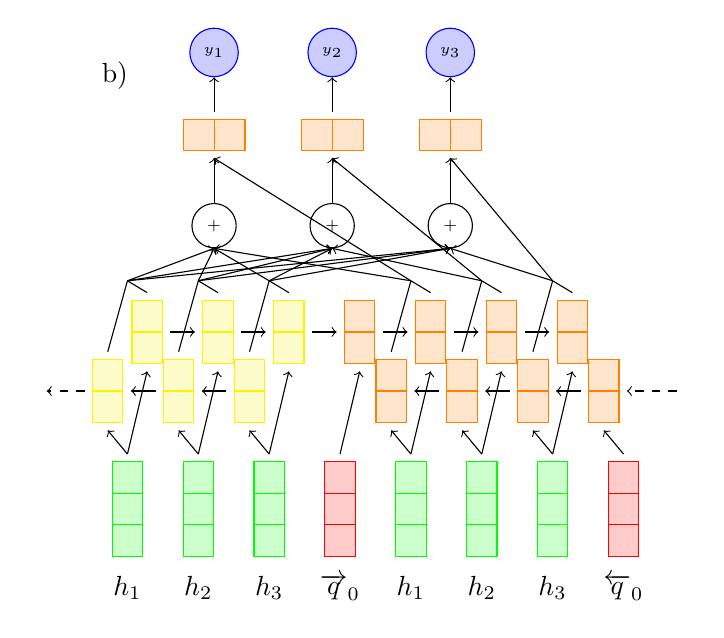
\begin{tikzpicture}[
  hid/.style 2 args={
    rectangle split,
    draw=#2,
    rectangle split parts=#1,
    fill=#2!20,
    outer sep=1mm},
  mlp/.style 2 args={
    rectangle split,
    rectangle split horizontal,
    draw=#2,
    rectangle split parts=#1,
    fill=#2!20,
    outer sep=1mm}
]

  \node [anchor=west] (label) at (.45, 4.5) {b)};

  \foreach \i [count=\step from 1] in {$h_1$, $h_2$, $h_3$} {
    \node (i\step) at (.9*\step, -2) {\i};
    \node[hid={3}{green}] (e\step) at (.9*\step, -1) {};    
  }
  \node (i4) at (.9*4, -2) {$\overrightarrow{q}_0$};
  \node[hid={3}{red}] (e4) at (.9*4, -1) {};    
  \foreach \i [count=\step from 5] in {$h_1$, $h_2$, $h_3$} {
    \node (i\step) at (.9*\step, -2) {\i};
    \node[hid={3}{green}] (e\step) at (.9*\step, -1) {};    
  }
  \node (i8) at (.9*8, -2) {$\overleftarrow{q}_0$};
  \node[hid={3}{red}] (e8) at (.9*8, -1) {};    

  \foreach \step in {1,...,3} {
    \node[hid={2}{yellow}] (h_r_\step) at (-.25 + .9 *\step, .5) {};    
    \node[hid={2}{yellow}] (h_f_\step) at (.25 + .9 *\step, 1.25) {};    
    \draw[->] (e\step.north) -> (h_f_\step.south);
    \draw[->] (e\step.north) -> (h_r_\step.south);
%    \node[mlp={2}{yellow}] (h_\step) at (.9 *\step, 2.5) {};    
%    \node[circle, draw=blue, fill=blue!20] (y_\step) at (.9 *\step, 3.75) {$y_\step$};    
%    \draw[->] (h_\step.north) -> (y_\step.south);
%    \draw[->] (h_f_\step.north) -> (h_\step.south);
%    \draw[->] (h_r_\step.north) -> (h_\step.south);
  }

  \foreach \step in {5,...,8} {
    \node[hid={2}{orange}] (h_r_\step) at (-.25 + .9 *\step, .5) {};    
    \draw[->] (e\step.north) -> (h_r_\step.south);
  }
  \foreach \step in {4,...,7} {
    \node[hid={2}{orange}] (h_f_\step) at (.25 + .9 *\step, 1.25) {};    
    \draw[->] (e\step.north) -> (h_f_\step.south);
%    \draw[->] (e\step.north) -> (h_r_\step.south);
%    \node[mlp={2}{yellow}] (h_\step) at (.9 *\step, 2.5) {};    
%    \node[circle, draw=blue, fill=blue!20] (y_\step) at (.9 *\step, 3.75) {$y_\step$};    
%    \draw[->] (h_\step.north) -> (y_\step.south);
%    \draw[->] (h_f_\step.north) -> (h_\step.south);
%    \draw[->] (h_r_\step.north) -> (h_\step.south);

  }

  \draw[->] (h_f_1.east) -> (h_f_2.west);
  \draw[->] (h_f_2.east) -> (h_f_3.west);
  \draw[->] (h_f_3.east) -> (h_f_4.west);
  \draw[->] (h_f_4.east) -> (h_f_5.west);
  \draw[->] (h_f_5.east) -> (h_f_6.west);
  \draw[->] (h_f_6.east) -> (h_f_7.west);
 
  \draw[->] (h_r_3.west) -> (h_r_2.east);
  \draw[->] (h_r_2.west) -> (h_r_1.east);
  \node (lborder) at (-.25 + .9 * 0, .5) {};
  \node (rborder) at (-.1 + .9 * 9, .5) {};
  \draw[->,dashed] (h_r_1.west) -- (lborder);
  \draw[->,dashed] (rborder) -- (h_r_8.east);
  \draw[->] (h_r_8.west) -> (h_r_7.east);
  \draw[->] (h_r_7.west) -> (h_r_6.east);
  \draw[->] (h_r_6.west) -> (h_r_5.east);

  \node[circle,draw=black] (attn1) at (2, 2.6) {\tiny$+$};    
  \node[circle,draw=black] (attn2) at (3.5, 2.6) {\tiny$+$};    
  \node[circle,draw=black] (attn3) at (5, 2.6) {\tiny$+$};    
  
  \node[mlp={2}{orange}] (h1) at (2, 3.75) {};
  \node[mlp={2}{orange}] (h2) at (3.5, 3.75) {};
  \node[mlp={2}{orange}] (h3) at (5, 3.75) {};
  \node[circle, draw=blue, fill=blue!20] (y1) at (2, 4.8) {\tiny $y_1$};    
  \node[circle, draw=blue, fill=blue!20] (y2) at (3.5, 4.8) {\tiny $y_2$};    
  \node[circle, draw=blue, fill=blue!20] (y3) at (5, 4.8) {\tiny $y_3$};    

  \foreach \step in {1,...,3} {
      \node (m\step) at (\step * .9, 1.9) {};
      \path[draw=black,-] (h_f_\step.north) -- (m\step.center);
      \path[draw=black,-] (h_r_\step.north) -- (m\step.center);
      \foreach \stepj in {1,...,3} {
          \path[draw=black,->] (m\step.center) -- (attn\stepj.south);
      } 
  }

  \foreach \step in {1,...,3} {
      \path[draw=black,->] (attn\step.north) -- (h\step.south);
      \path[draw=black,->] (h\step.north) -- (y\step.south);
  }


  \node (m21) at (5* .9, 1.9) {};
  \path[draw=black,-] (h_f_5.north) -- (m21.center);
  \path[draw=black,-] (h_r_5.north) -- (m21.center);
  \path[draw=black,->] (m21.center) -- (attn1.south);
  \path[draw=black,->] (m21.center) -- (h1.south);

  \node (m22) at (6* .9, 1.9) {};
  \path[draw=black,-] (h_f_6.north) -- (m22.center);
  \path[draw=black,-] (h_r_6.north) -- (m22.center);
  \path[draw=black,->] (m22.center) -- (attn2.south);
  \path[draw=black,->] (m22.center) -- (h2.south);


  \node (m23) at (7* .9, 1.9) {};
  \path[draw=black,-] (h_f_7.north) -- (m23.center);
  \path[draw=black,-] (h_r_7.north) -- (m23.center);
  \path[draw=black,->] (m23.center) -- (attn3.south);
  \path[draw=black,->] (m23.center) -- (h3.south);




\end{tikzpicture}


\end{document}

%        \end{column}
%        \begin{column}{0.5\textwidth}
%            \begin{align*}
%                p(y|h) &= \prod_{i=1}^n p(y_i|h)\\
%                p(y_i|h) &= \sigma\left(W \left[ \begin{array}{l} h_i^{(d)}\\
%         \tilde{h}_i \end{array} \right]    + b \right) \\
%         \tilde{h}_i & = \sum_{j=1}^{n} \alpha_{i,j} \cdot h^{(e)}_j\\
%         \alpha_{i,j} & = \operatorname{Softmax}(h^{(e)}  \cdot h^{(d)}_i)_j \\
%            & \propto \exp\left(h^{(e)}_j  \cdot h^{(d)}_i \right) \\
%            \end{align*}
%        \end{column}
%    \end{columns}
%\end{frame}
%
%\begin{frame}{Cheng \& Lapata Extractor}
%  \begin{columns}
%    \begin{column}{0.5\textwidth}
%        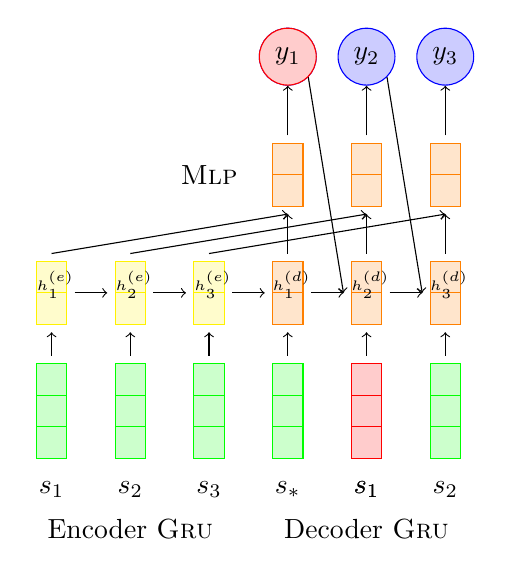
\begin{tikzpicture}[
  hid/.style 2 args={
    rectangle split,
    draw=#2,
    rectangle split parts=#1,
    fill=#2!20,
    outer sep=1mm},
  mlp/.style 2 args={
    rectangle split,
    rectangle split horizontal,
    draw=#2,
    rectangle split parts=#1,
    fill=#2!20,
    outer sep=1mm}
]

 \foreach \i [count=\step from 1] in {$s_1$, $s_2$, $s_3$, $s_*$, $s_1$, $s_2$}
    \node (i\step) at (1*\step, -2) {\i};
  % draw embedding and hidden layers for text input
  \foreach \step in {1,...,3} {
    \node[hid={3}{green}] (e\step) at (1*\step, -1) {};    
  }
    \node[hid={3}{green}] (e4) at (1*4, -1) {};    
  \foreach \step in {5,...,6} {
    \node[hid={3}{green}] (e\step) at (1*\step, -1) {};    
  }

  \foreach \step in {1,...,3} {
    \node[hid={2}{yellow}] (h_f_\step) at (1 *\step, .5) {};    
    \draw[->] (e\step.north) -> (h_f_\step.south);
  }

  \foreach \step in {1,...,3} {
      \node (hlbl\step) at (1*\step + .05, .6) {\tiny $h^{(e)}_\step$};    
  }


  \foreach \step in {4,...,6} {
    \node[hid={2}{orange}] (h_f_\step) at (1 *\step, .5) {};    
    \node[hid={2}{orange}] (g_f_\step) at (1 *\step, 2) {};    
    \draw[->] (e\step.north) -> (h_f_\step.south);
  }

  \foreach \step in {1,...,3} {
      \node (hlbl\step) at (1*\step + 3 + .05, .6) {\tiny $h^{(d)}_\step$};    
  }
  \foreach \step in {1,...,3} {
    \node[circle, draw=blue, fill=blue!20] (y_\step) at (3 + 1 *\step, 3.5) {$y_\step$};    
 }
    \draw[->] (y_1.south east) -> (h_f_5.west);
    \draw[->] (y_2.south east) -> (h_f_6.west);
    \draw[->] (h_f_4.north) -> (g_f_4.south);
    \draw[->] (g_f_4.north) -> (y_1.south);
    \draw[->] (h_f_5.north) -> (g_f_5.south);
    \draw[->] (g_f_5.north) -> (y_2.south);
    \draw[->] (h_f_6.north) -> (g_f_6.south);
    \draw[->] (g_f_6.north) -> (y_3.south);
 \foreach \step/\steppp in {1/2, 2/3, 3/4, 4/5, 5/6} {
   
    \draw[->] (h_f_\step.east) -> (h_f_\steppp.west);
  }
    \draw[->] (h_f_1.north) -> (g_f_4.south);
    \draw[->] (h_f_2.north) -> (g_f_5.south);
    \draw[->] (h_f_3.north) -> (g_f_6.south);

    \node (enc) at (2,-2.5) {Encoder \textsc{Gru}};
    \node (dec) at (5,-2.5) {Decoder \textsc{Gru}};
    \node (mlp) at (3, 2) {\textsc{Mlp}};

  \uncover<5->{
  \node (i5) at (1*5, -2) {\alert{$s_1$}};
    \node[circle, draw=red, fill=red!20] (y_1) at (3 + 1 *1, 3.5) {$y_1$};    
    \node[hid={3}{red}] (e5) at (1*5, -1) {};    
}

\end{tikzpicture}

%    \end{column}
%    \begin{column}{0.5\textwidth}
%      \begin{align*}
%        \uncover<1->{p(y|h) &= \prod_{i=1}^n p(y_i|y_{<i}, h^{(d)}_{<i}, 
%                                                       h^{(e)} )}\\
%        \uncover<2->{p_i & \triangleq p(y_i=1|h) = 
%                            \textsc{Mlp}([h^{(e)}_i; h^{(d)}_i])}\\
%        \uncover<3->{h^{(d)}_i &= \textsc{Gru}\left(h_{i-1}^{(d)},  
%                                 \alert<5->{p_{i-1} \cdot  s_{i-1}}\right)}
%      \end{align*}
%    \end{column}
%  \end{columns}
%\end{frame}
%
%\begin{frame}{Sentence Extractor}
%  \textbf{Previous Work}\\~\\
%  ~~ -- \textbf{Cheng and Lapata Extractor} ~~ seq2seq inspired architecture 
%                                               (Cheng and Lapata, 2016)\\
%  ~~ -- \alert{\textbf{SummaRunner Extractor}} ~~ RNN inspired architecture 
%                                                  with document and summary 
%                                                  representations 
%                                                  (Nallapati et al., 2016)\\
%  ~\\~\\
%  \textbf{Our Extractors}\\~\\
%  ~~ -- \textbf{RNN Extractor} ~~ Simplified version of SummaRunner \\
%  ~~ -- \textbf{Seq2Seq Extractor} ~~ seq2seq (with attention) inspired 
%                                      architecture \\
%\end{frame}
%
%
%
%\begin{frame}{SummaRunner Extractor}
%  \begin{columns}
%    \begin{column}{0.5\textwidth}
%      \documentclass[tikz,border=10pt]{standalone}
\usetikzlibrary{shapes}
\usetikzlibrary{arrows}
\usetikzlibrary{positioning}
\begin{document} 

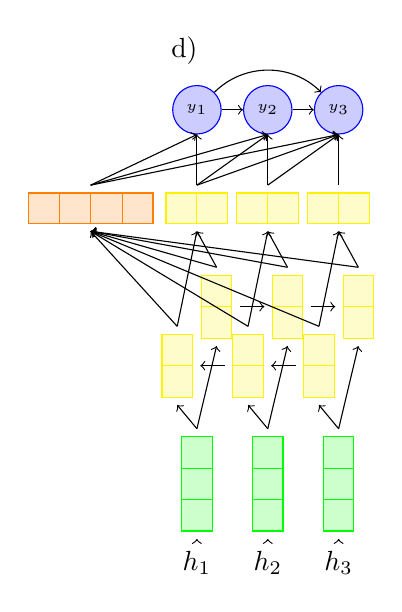
\begin{tikzpicture}[
  hid/.style 2 args={
    rectangle split,
    draw=#2,
    rectangle split parts=#1,
    fill=#2!20,
    outer sep=1mm},
  mlp/.style 2 args={
    rectangle split,
    rectangle split horizontal,
    draw=#2,
    rectangle split parts=#1,
    fill=#2!20,
    outer sep=1mm}
]

  \node [anchor=west] (label) at (.45, 4.5) {d)};
 \foreach \i [count=\step from 1] in {$h_1$, $h_2$, $h_3$}
    \node (i\step) at (.9*\step, -2) {\i};
  % draw embedding and hidden layers for text input
  \foreach \step in {1,...,3} {
    \node[hid={3}{green}] (e\step) at (.9*\step, -1) {};    
    \draw[->] (i\step.north) -> (e\step.south);
  }

        \node[mlp={4}{orange}] (h_0) at (.9 *-.5, 2.5) {};    
  \foreach \step in {1,...,3} {
    \node[hid={2}{yellow}] (h_f_\step) at (.25 + .9 *\step, 1.25) {};    
    \node[hid={2}{yellow}] (h_r_\step) at (-.25 + .9 *\step, .5) {};    
    \draw[->] (h_r_\step.north) -> (h_0.south);
    \draw[->] (h_f_\step.north) -> (h_0.south);
    \draw[->] (e\step.north) -> (h_f_\step.south);
    \draw[->] (e\step.north) -> (h_r_\step.south);
    \node[mlp={2}{yellow}] (h_\step) at (.9 *\step, 2.5) {};    
    \node[circle, draw=blue, fill=blue!20] (y_\step) at (.9 *\step, 3.75) {\tiny $y_\step$};    
    \draw[->] (h_\step.north) -> (y_\step.south);
    \draw[->] (h_f_\step.north) -> (h_\step.south);
    \draw[->] (h_r_\step.north) -> (h_\step.south);
  }

  \foreach \step/\steppp in {1/2, 2/3} {
    \draw[->] (h_f_\step.east) -> (h_f_\steppp.west);
    \draw[->] (h_r_\steppp.west) -> (h_r_\step.east);
  }
 
    \draw[->] (h_0.north) -> (y_1.south);
    \draw[->] (h_0.north) -> (y_2.south);
    \draw[->] (h_0.north) -> (y_3.south);
    \draw[->] (y_1.east) -> (y_2.west);
    \draw[->] (y_2.east) -> (y_3.west);
    \draw[->] (h_1.north) -> (y_2.south);
    \draw[->] (h_1.north) -> (y_3.south);
    \draw[->] (h_2.north) -> (y_3.south);
    \draw [bend left=45,->] (y_1) to (y_3);
\end{tikzpicture}


\end{document}

%    \end{column}
%    \begin{column}{0.5\textwidth}
%      $d = \tanh\big(b_d + W_d \frac{1}{n} \sum_{i=1}^n h_i   \big) $\\
%      $ g_i  = \sum_{j=1}^{i-1} p(y_j=1|y_{<j},h) \cdot h_j$\\
%      \begin{align*}
%        \textit{content}  \quad a^{(con)}_i & =W^{(con)} h_i \\
%        \textit{salience} \quad a^{(sal)}_i & = h_i^TW^{(sal)} d \\
%        \textit{novelty} \quad a^{(nov)}_i & = -h_i^TW^{(nov)} \tanh(g_i) 
%                    \label{eq:srnov} \\
%        \textit{position} \quad a^{(pos)}_i & = W^{(pos)} l_i \\
%        \textit{quartile} \quad a^{(qrt)}_i & = W^{(qrt)} r_i
%      \end{align*}
%      $p(y_i|y_{<i}, h) = \sigma\left(\begin{array}{l} a^{(con)}_i 
%        +a^{(sal)}_i + a^{(nov)}_i+ \\ a^{(pos)}_i + a^{(qrt)}_i + 
%         b \end{array}\right) $ \\
%    \end{column}
%  \end{columns}
%\end{frame}


